\chapter{Code Structure}
\label{cha:structure}
\section{Structure}
As said in the DD, to address the issue of maximizing the code sharing, our application project is based on a \textit{Portable Class Library} (PCL), which means that the main solution consists of a Core PCL project, which contains all the pages (\textit{Views}) and, mostly for each page, its counterpart of business logic (\textit{ViewModels}) and two other platform-specific projects. The latter, specifically for iOS and Android, contain anything that must be written for a specific platform. This typically consists of renderers, a way that Xamarin.Forms provides to developers to customize the appearance and behavior of Xamarin.Forms controls on each platform and handle native elements differently, and other code which is platform-dependent. So, the majority of the functionalities, wrapped in classes, are located in the PCL project, which shares the business logic across the implementation and the customization is left to the platform-specific projects. \\

The PCL consists of two folders, the \textit{AppCore} and the \textit{Framework} ones, which contains respectively the implementation of the core logic and the abstract classes or interfaces that are implemented by the PCL itself or the platform projects, and \textit{App.cs}, the entrypoint of the application. Again, we respected the choices mentioned in the DD, which means that, having used the MVVM architectural pattern, not only we tried to maximize the code sharing implementing almost all the functionalities we were requested to - with a great focus on quality too -, but we achieved separation of concerns and used platform code through the dependency service as well. \\

Each of the two platform-related projects includes a \textit{Dependencies} folder that contains the platform implementations of the platform functionality needed to be shared. An example could be the implementation of the Toast notification (a non-annoying pop-up which mainly informs users that something went wrong), natively present on Android but not on iOS (so it has been implemented on iOS too). The other folder are, as said, the so called \textit{Renderers}, which implements a native UI element changing the normal view of the Xamarin.Form element in something specifically customized for the platform. Here's an example too: the secondary toolbar, which is the navigation bar that includes all the main buttons such as \textit{Today}, \textit{Tickets} and so on, is perfectly rendered on Android through the pop-up button (the three dots button). On iOS, however, such bar is not rendered at all, and, at the time of writing, has not been implemented by Xamarin.Forms yet. So we created it by ourselves, directly with native iOS API. As can be seen from the renderers, code has been highly customized to achieve also a friendly and pretty user interface. Figure \ref{fig:structure} shows how the code has been laid out.

\begin{figure}
	\centering
	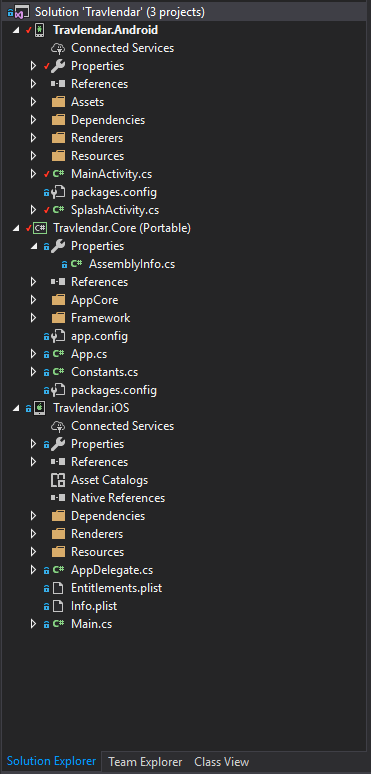
\includegraphics[width=4in]{./images/code_structure.png}
	\caption{Code Structure.}
	\label{fig:structure}
\end{figure}
